\chapter{TINJAUAN PUSTAKA}
\label{chap:tinjauanpustaka}
\section{Penelitian Terdahulu}
\label{sec:penelitianterdahulu}
\subsection{2D Cam Capture: An Optimal Real-TimeDimension Measurement System}
\label{subsec:2Dmeasure}

Pada tahun 2019 terdapat paper yang mengerjakan suatu pemrosesan gambar untuk mengukur luas suatu bangun datar 2 dimensi yang pengaplikasiannya dalam bentuk bahan tekstil. metode yang digunakan adalah dengan algoritma cam capture 2D menggunakan urutan gambar gambar teknik pengolahan. Ini memudahkan proses pengukuran dengan memberikan dimensi yang akurat dari berbagai bentuk tana distorsi. sistem berbasis visi komuter ini melibatkan penangkapan gambar, pemrosesan, dan analisis bentuk menggunakan perhitungan piksel algoritma sehingga memberikan pengukuran yang akurat\citep{2Dmeasure}. pada penelitian sebelumnya dilakukan perhitungan luas daripada objek dua dimensi yang bentuknya tidak beraturan, untuk penelitian yang saya lakukan adalah menghitung luas bangun datar pada papan tulis dengan menggunakan metode YOLO.

\section{Bangun Datar}
\label{subsec:BangunDatar}
Dalam geometri, bentuk 2D didefinisikan sebagai bangun datar yang hanya memiliki dua dimensi yaitu panjang dan lebar. Mereka tidak memiliki ketebalan apapun dan hanya dapat diukur dengan dua dimensi. Lingkaran, persegi, persegi panjang, dan segitiga adalah beberapa contoh benda dua dimensi dan bentuk-bentuk ini dapat digambar di atas kertas. Semua bentuk 2D memiliki sisi, simpul (sudut), dan sudut internal, kecuali lingkaran, yang merupakan sosok melengkung. Bentuk 2D dengan setidaknya tiga sisi lurus disebut poligon dan itu termasuk segitiga, bujur sangkar, dan segi empat.\citep{BRIBIESCA1992483}

\subsection{Segitiga}
Segitiga adalah poligon dengan tiga sisi dan tiga simpul. Ini adalah salah satu bentuk dasar dalam geometri. Dalam geometri Euclidean, setiap tiga titik, ketika non-collinear, menentukan segitiga unik dan secara bersamaan, bidang unik (yaitu ruang Euclidean dua dimensi). Dengan kata lain, hanya ada satu bidang yang memuat segitiga tersebut, dan setiap segitiga terdapat pada suatu bidang. Jika seluruh geometri hanya bidang Euclidean, hanya ada satu bidang dan semua segitiga terkandung di dalamnya; namun, dalam ruang Euclidean berdimensi lebih tinggi, hal ini tidak lagi benar. Setiap segitiga memiliki tiga sisi dan tiga sudut, beberapa di antaranya mungkin sama. Sisi segitiga diberi nama khusus dalam kasus segitiga siku-siku, dengan sisi di depan sudut siku-siku disebut sisi miring dan dua sisi lainnya dikenal sebagai kaki. Semua segitiga adalah cembung dan bisentris. Bagian dari bidang yang dilingkupi segitiga itu disebut bagian dalam segitiga, sedangkan bagian luarnya adalah bagian luar.\citep{segitiga}
\setlength{\belowcaptionskip}{-5pt}
\begin{center}
	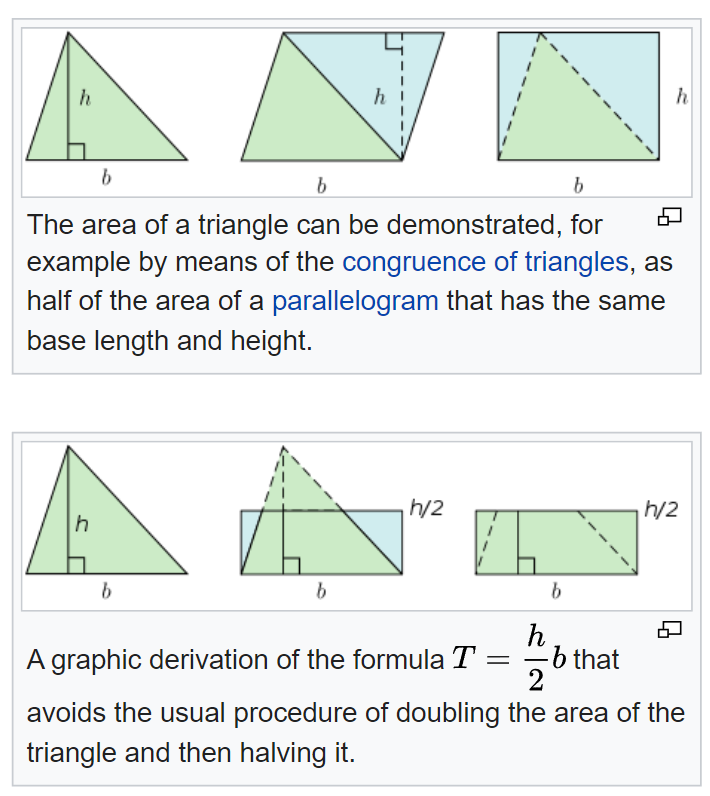
\includegraphics[width=0.65\textwidth]{gambar/luassegitiga.png}
	\captionof{figure}{Luas Segitiga}
\end{center}
Menghitung luas segitiga dapat dengan menggunakan rumus $T = \frac{1}{2} bh$, di mana b adalah panjang alas segitiga, dan h adalah tinggi atau tinggi segitiga. Istilah "alas" menunjukkan sisi mana pun, dan "tinggi" menunjukkan panjang tegak lurus dari titik di seberang alas ke garis yang memuat alas. Meskipun sederhana, rumus ini hanya berguna jika tinggi dan alasnya dapat dengan mudah ditemukan.\citep{segitiga}

\subsection{Persegi}
Istilah "persegi" dapat digunakan untuk mengartikan bilangan kuadrat ("$x^2$ adalah kuadrat dari $x$") atau bangun geometri yang terdiri dari segi empat cembung dengan sisi-sisi yang sama panjang yang ditempatkan pada sudut siku-siku satu sama lain, dengan kata lain, persegi adalah poligon beraturan dengan empat sisi.\citep{Squarefr70:online}
\begin{center}
	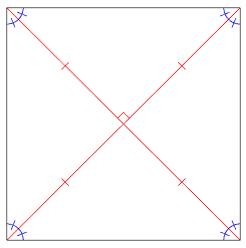
\includegraphics[width=0.35\textwidth]{gambar/persegipustaka.png}
	\captionof{figure}{Ilustrasi Persegi}
\end{center}
Diagonal persegi saling membagi dua dan tegak lurus (diilustrasikan dengan warna merah pada gambar di atas). Selain itu, mereka membagi dua setiap pasangan sudut yang berlawanan (diilustrasikan dengan warna biru).\citep{Squarefr70:online}
\begin{center}
	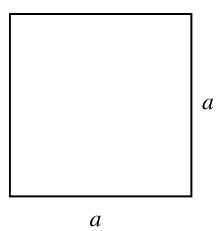
\includegraphics[width=0.35\textwidth]{gambar/Square_1000.png}
	\captionof{figure}{Ilustrasi Luas Persegi}
\end{center}
Untuk mencari luas persegi A dapat menggunakan rumus $A = a^2$.\citep{Squarefr70:online}

\subsection{Lingkaran}
Lingkaran adalah himpunan titik-titik pada bidang yang berjarak sama dari suatu titik O. Jarak r dari pusat disebut jari-jari, dan titik O disebut pusat. Jari-jari dua kali dikenal sebagai diameter $d = 2r$. Sudut yang dibentuk lingkaran dari pusatnya adalah sudut penuh, sama dengan $360\degree$ atau $2\pi$ radian.\citep{Circlefr27:online}
\begin{center}
	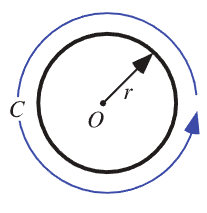
\includegraphics[width=0.35\textwidth]{gambar/lingkaranpustaka.png}
	\captionof{figure}{Ilustrasi Lingkaran}
\end{center}
Sebuah lingkaran memiliki luas maksimum yang mungkin untuk keliling tertentu, dan keliling minimum yang mungkin untuk luas tertentu. Keliling C suatu lingkaran disebut keliling, dan diberikan oleh $C = \pi d = 2\pi r$.\citep{Circlefr27:online}
\begin{center}
	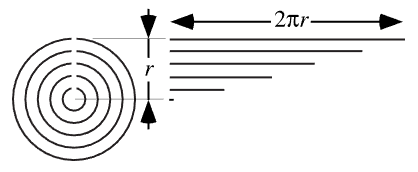
\includegraphics[width=0.50\textwidth]{gambar/luaslingkaranpustaka.png}
	\captionof{figure}{Ilustrasi Luas Lingkaran}
\end{center}
Mengetahui C/d, luas lingkaran dapat dihitung baik secara geometris atau menggunakan kalkulus. Ketika jumlah strip konsentris meningkat hingga tak terhingga seperti yang digambarkan di atas, mereka membentuk segitiga, maka luas lingkaran A adalah $A = \frac{1}{2} (2\pi r)r = \pi r^2$.\citep{Circlefr27:online}

\subsection{Persegi Panjang}
\begin{center}
	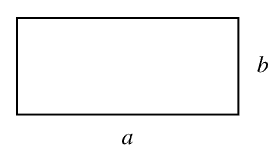
\includegraphics[width=0.50\textwidth]{gambar/persegipanjangpustaka.png}
	\captionof{figure}{Ilustrasi Peregi Panjang}
\end{center}
Persegi panjang adalah segi empat planar tertutup dengan sisi-sisi yang berhadapan sama panjang a dan b, dan dengan empat sudut siku-siku. Persegi adalah persegi panjang yang mengalami degenerasi dengan $a = b$. Luas persegi panjang adalah $A = ab$.\citep{Rectangl23:online}

\subsection{Trapesium}
\begin{center}
	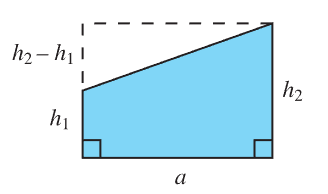
\includegraphics[width=0.50\textwidth]{gambar/trapesiumpustaka.png}
	\captionof{figure}{Ilustrasi Trapesium}
\end{center}
Sebuah segi empat dengan setidaknya satu pasang sisi sejajar, trapesium harus merupakan segiempat cembung dalam geometri Euclidean. Sisi-sisi yang sejajar disebut alas trapesium. Dua sisi lainnya disebut kaki (atau sisi lateral).\citep{RightTra69:online}\\
Luas trapesium A dapat dihitung dengan cara $A = a h_2 - \frac{1}{2} (h_2 - h_1) a = \frac{1}{2} a(h_1 + h_2)$.\citep{RightTra69:online}

\section{Visi Komputer}
Computer Vision (CV) adalah salah satu teknologi Artificial Intelligence yang hadir di banyak aplikasi AI yang kita temui. Pengenalan wajah, mobil self-driving, augmented reality dan banyak lagi aplikasi memanfaatkan teknik visi komputer dalam beberapa bentuk. Selama dekade terakhir, visi komputer menjadi lebih menonjol karena aplikasi AI mendapatkan lebih banyak adopsi. Peningkatan adopsi aplikasi AI berkontribusi pada peningkatan jumlah pekerjaan dan kursus terkait visi komputer. Sistem sensorik penglihatan manusia telah berkembang selama ribuan tahun untuk memberi manusia kemampuan untuk memperkirakan makna dan konteks pemandangan dari cahaya yang dipantulkan oleh objek di dunia 3 dimensi kita, ke mata kita. Mata dan otak kita dapat menyimpulkan pemahaman tentang lingkungan dari cahaya yang dipantulkan. Sistem visual kita membekali kita dengan kemampuan untuk menentukan jarak objek, memprediksi tekstur objek tanpa bersentuhan langsung, dan mengidentifikasi segala macam pola dan kejadian di lingkungan kita. Computer Vision adalah proses di mana kami mencoba untuk melengkapi sistem komputer dengan kemampuan yang sama yang dimiliki sistem sensor visual manusia. Definisi yang tepat untuk computer vision adalah sebagai berikut: Computer Vision adalah proses dimana mesin atau sistem menghasilkan pemahaman informasi visual dengan menerapkan satu atau lebih algoritma yang bekerja pada informasi yang diberikan. Pemahaman tersebut kemudian diterjemahkan ke dalam keputusan, klasifikasi, pengamatan pola, dan banyak lagi. Sistem sensorik visual kita terdiri dari mata dan otak, meskipun kita memahami bagaimana setiap komponen mata seperti kornea, lensa, retina, Iris, dll., Kita tidak sepenuhnya memahami cara kerja otak. Untuk membuat algoritma dan sistem yang memiliki kemampuan mengekstrak informasi kontekstual dari gambar, penyebab pola harus diamati. Kemudian solusi dapat diturunkan dari pemahaman tentang sebab dan akibat dari pola-pola tertentu.\citep{ABeginne17}\\
Contoh kegunaan visi komputer adalah sebagai berikut:

\begin{center}
	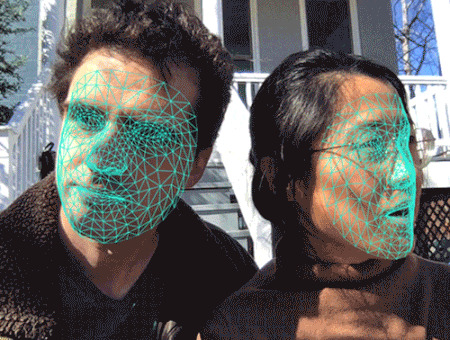
\includegraphics[width=0.70\textwidth]{gambar/face.jpg}
	\captionof{figure}{\textit{face detection}\citep{ABeginne17}}
\end{center}
Deteksi Wajah: Tugas menerapkan sistem yang dapat secara otomatis mengenali dan melokalisasi wajah manusia dalam gambar dan video. Deteksi wajah hadir dalam aplikasi yang terkait dengan pengenalan wajah, fotografi, dan penangkapan gerak.\citep{ABeginne17}
\begin{center}
	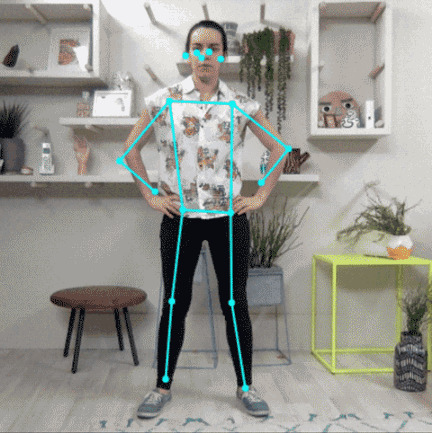
\includegraphics[width=0.50\textwidth]{gambar/body.jpg}
	\captionof{figure}{\textit{Estimasi Pose}\citep{ABeginne17}}
\end{center}
Estimasi Pose: Proses menyimpulkan lokasi sendi utama tubuh dari aset digital yang disediakan seperti gambar, video, atau urutan gambar. Bentuk estimasi pose hadir dalam aplikasi seperti pengenalan tindakan, interaksi manusia, penciptaan aset untuk realitas virtual dan permainan grafis 3D, robotika dan banyak lagi.\citep{ABeginne17}
\begin{center}
	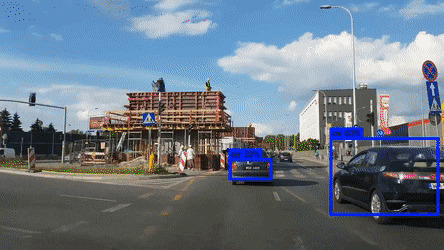
\includegraphics[width=0.70\textwidth]{gambar/car.jpg}
	\captionof{figure}{\textit{Deteksi Objek}\citep{ABeginne17}}
\end{center}
Pelacakan Objek: Metode untuk mengidentifikasi, mendeteksi, dan mengikuti objek yang diinginkan dalam urutan gambar selama beberapa waktu. Aplikasi pelacakan dalam sistem ditemukan di banyak kamera pengintai dan perangkat pemantauan lalu lintas.\citep{ABeginne17}
Klasifikasi Objek: Proses mengidentifikasi kelas yang dikaitkan dengan objek target. Pengenalan dan deteksi objek adalah teknik dengan hasil dan pendekatan implementasi yang serupa, meskipun proses pengenalan datang sebelum langkah-langkah deteksi dalam berbagai sistem dan algoritma.\citep{ABeginne17}

Sejak tahun 1970-an para peneliti telah menghabiskan banyak waktu dan tenaga, menciptakan algoritma dan sistem visi komputer yang efisien dan kuat yang dapat digunakan sebagai solusi untuk beberapa aplikasi yang tercantum di atas. Di zaman modern, sebagian besar tugas visi komputer diselesaikan menggunakan pendekatan Deep Learning.\citep{ABeginne17}

\section{Deep Learning}
\label{subsec:DeepLearning}
Deep learning memungkinkan model komputasi yang terdiri dari beberapa lapisan pemrosesan untuk mempelajari representasi data dengan berbagai tingkat abstraksi. Metode-metode ini telah secara dramatis meningkatkan state-of-the-art dalam pengenalan suara, pengenalan objek visual, deteksi objek dan banyak domain lainnya seperti penemuan obat dan genomik. Deep learning menemukan struktur rumit dalam kumpulan data besar dengan menggunakan algoritma backpropagation untuk menunjukkan bagaimana mesin harus mengubah parameter internalnya yang digunakan untuk menghitung representasi di setiap lapisan dari representasi di lapisan sebelumnya. Deep convolutional nets telah menghasilkan terobosan dalam pemrosesan gambar, video, ucapan, dan audio, sedangkan jaring berulang telah menyoroti data berurutan seperti teks dan ucapan.\citep{article}

Deep Learning (DL) atau Pembelajaran Mendalam atau Belajar Secara
Mendalam adalah salah satu cabang dari Machine Learning yang
terdiri dari algoritma pemodelan abstraksi tingkat tinggi pada data
menggunakan sekumpulan fungsi transformasi non-linear yang ditata
berlapis-lapis dan mendalam. DL sangat baik untuk diterapkan pada
supervised learning, unsupervised learning dan semi-supervised
learning maupun untuk reinforcement learning dalam berbagai
aplikasi seperti pengenalan citra, suara, klasifikasi teks, dan
sebagainya. Model pada DL pada dasarnya dibangun berdasarkan Jaringan
saraf tiruan (Neural Network), yang risetnya sudah berlangsung sejak
era 80an namun baru-baru ini kembali bangkit dengan adanya
komputer yang semakin cepat apalagi ditambah dengan adanya
teknologi pada Big Data, misal pada hadoop dan spark berbasis multi
node cluster, maupun pemrosesan secara paralel berbasis GPU.\citep{bookDL}

Deep Learning merupakan pembelajaran yang berbasis pada
fitur yang berbentuk hirarki, yang mana bentuk fitur hirarki tersebut
dapat diskalakan dalam ukuran tertentu yang dapat disesuaikan
dengan kasus yang diproses. Sehingga membuat algoritma Deep
Learning mampu untuk melakukan ekstraksi fitur otomatis dari data
mentah secara detail, karena proses ekstraksi yang dilakukan
menggunakan struktur eksploitasi, dimana fitur-fitur yang
dieksploitasi tersebut tidak mungkin dapat dilihat secara kasat mata.
Hal ini dikarenakan distribusi pembeda kelas data biasanya terlalu
dalam, sehingga dari fitur level tinggi harus ditransformasi terlebih
dahulu ke fitur yang paling rendah yang dapat mudah dipahami oleh
mesin pembelajaran. Artinya jika fitur level rendah saja dapat mudah
diindentifikasi oleh Deep Learning, apalagi yang fitur level tinggi.
Perpaduan inilah yang menjadikan Deep Learning mampu
menghasilkan representasi fitur yang baik dan optimal. Penggalian
fitur secara eksploitasi ini mencoba untuk mengolah suatu space atau
region pada posisi tertentu sampai dicoba untuk digali dan difilter
sampai sedalam-dalamnya. Sedangkan jika secara eksplorasi, Deep
Learning berusaha untuk mengumpulkan target spae atau region
sebanyak-banyaknya atau seluas-luasnya dengan teknik yang bisa
sama atau berbeda pada saat melakukan eksplotasi. Berikut adalah
prinsip kerja dari algoritma Deep Learning.\citep{bookDL}

\section{\textit{You Only Look Once (YOLO)}}
\label{subsec:YOLO}
YOLO (You Only Look Once) merupakan sistem deteksi objek secara waktu nyata. YOLO merupakan single CNN (Convulotional Neural Network) yang secara bersamaan memprediksi lebih dari satu bounding boxes dan kelas pada satu gambar dalam satu kali pindai. Framework ini dikembangkan oleh Redmon J., Divvala S., Girshick R., Farhadi A. arsitektur jaringannya terinspirasi dari model GoogLeNet untuk klasifikasi gambar. jaringan YOLO memiliki 24 convolutional layer diikuti dengan dua layer yang terhubung.
Saat ini, ada tiga versi YOLO yaitu YOLOv1, YOLOv2, dan YOLOv3. YOLOv2 merupakan versi yang telah dikembangkan dari YOLOv1 yang mana tetap memiliki kecepatan yang sama namun dengan penambahan batch normalization, anchor boxes dan high-resolution classifier. pada YOLOv3, fitur ektraksi yang lebih baik diperkenalkan dilanjutkan dengan perkenalan 53 convolutional layer terlatih pada ImageNet. Tingkat ketelitian YOLOv3 lebih baik dari YOLOv2 namun lebih lambat karena lebih banyak layer.\citep{Redmon_2016_CVPR}

Seperti pada Gambar \ref{fig:deteksi}, terdapat tiga langkah deteksi objek menggunakan YOLO seperti berikut:
\begin{enumerate}
	\item Mengubah ukuran dimensi masukan citra menjadi 448 × 448.
	\item Menjalankan single convolutional network pada citra.
	\item Melakukan threshold pada hasil deteksi berdasarkan nilai confidence yang didapatkan oleh model
\end{enumerate}

\begin{center}
	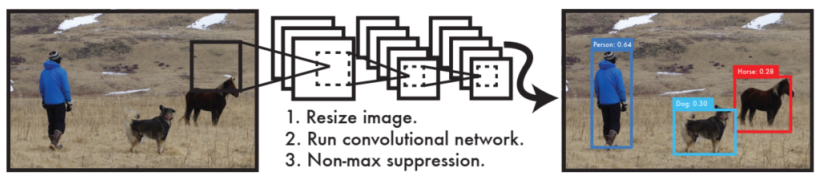
\includegraphics[width=0.75\textwidth]{gambar/deteksi.png}
	\captionof{figure}{Sistem Deteksi Pada YOLO}\citep{Redmon_2016_CVPR}
	\label{fig:deteksi}
\end{center}

Pada proses pertama, YOLO mendeteksi objek menggunakan unified detection yang menyatukan antara komponen deteksi objek kedalam single neural network. Desain YOLO memungkinkan end-toend training dan real-time speed dengan mempertahankan rata-rata
presisi yang tinggi. Sistem pada YOLO membagi gambar masukan
kedalam grid $S \times S$. Jika titik tengah dari sebuah objek terdapat
didalam salah satu sel, maka sel grid itu bertanggung jawab untuk
mendeteksi objek tersebut. Setiap sel kota memprediksi bounding
box B dan nilai confidence untuk setiap kotak. Nilai confidence
merepresentasikan keakuratan model bahwa terdapat objek dalam
bounding box tersebut\citep{Redmon_2016_CVPR}. Setiap bounding box memiliki 5 parameter
prediksi yaitu x, y, w, h, seperti pada Gambar \ref{fig:boundingbox} dan confidence.\citep{yolov3}
\begin{center}
	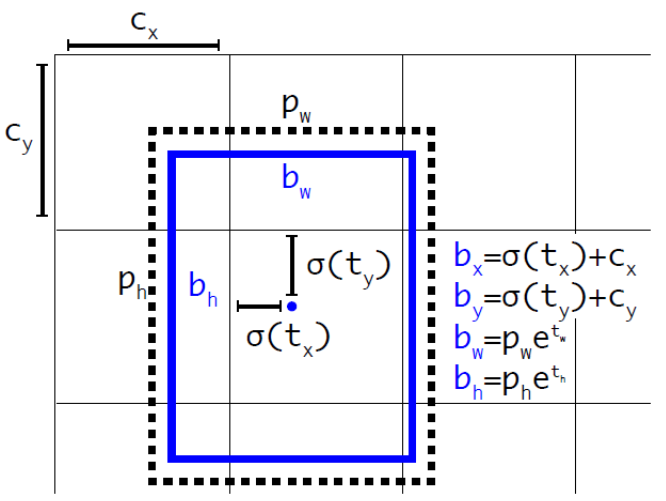
\includegraphics[width=0.75\textwidth]{gambar/boundingbox.png}
	\captionof{figure}{Bounding Box Pada YOLOv3}\citep{yolov3}
	\label{fig:boundingbox}
\end{center}

Koordinat (x,y) merupakan pusat dari kotak relatif ke gambar dan
confidence merupakan Intersection over Union (IoU) antara predicted box dengan ground-truth box. Setiap sel grid memprediksi
probabilitas kelas C. Setiap sel grid memprediksi nilai probabilitas
pada kelas C. Probabilitas tersebut dikondisikan berdasarkan sel
grid yang memuat objek. Sehingga hanya terdapat satu kelas probabilitas yang terdeteksi disetiap sel grid tanpa memperhitungkan
jumlah bounding box B. Saat deteksi, probabilitas kelas dikalikan
nilai confidence sesuai persamaan \ref{eq:1} atau disederhanakan menjadi seperti persamaan \ref{eq:2}.\citep{Redmon_2016_CVPR}
\begin{equation}\label{eq:1}
	Pr(Class_i|Object) \times Pr(Object) \times_{truth} IOU_{pred}
\end{equation}
\begin{equation}\label{eq:2}
	Pr(Class_i) \times_{truth} IOU_{pred}
\end{equation}

Dari persamaan tersebut, didapatkan nilai confidence dari kelas spesifik. Nilai ini merepresentasikan probabilitas kelas yang muncul didalam kotak dan seberapa baik kotak yang diprediksi akurat dengan
objek. Seperti pada ilustrasi pada Gambar \ref{fig:deteksi2}, YOLO mendeteksi
model sebagai regresi. Hal ini membagi gambar menjadi grid dan
secara bersamaan memprediksi bounding box dan confidence pada
bounding box tersebut dan kelas probabilitas.\citep{Redmon_2016_CVPR}

\begin{center}
	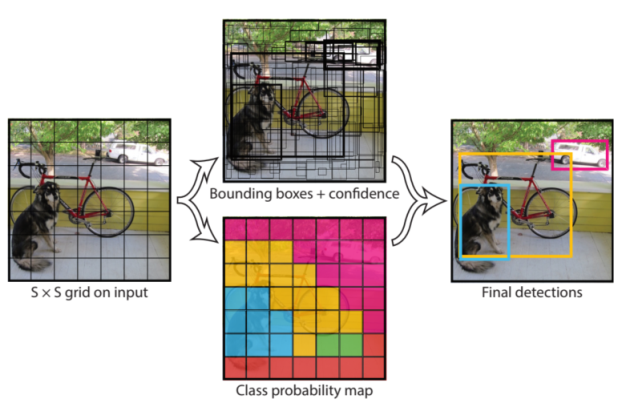
\includegraphics[width=0.75\textwidth]{gambar/deteksi2.png}
	\captionof{figure}{Proses Deteksi Pada YOLO}\citep{Redmon_2016_CVPR}
	\label{fig:deteksi2}
\end{center}

\subsection{\textit{YOLOv4-tiny}}
Metode Yolov4-tiny dirancang berdasarkan metode Yolov4 untuk membuatnya memiliki kecepatan deteksi objek yang lebih cepat. kecepatan deteksi objek untuk Yolov4-tiny dapat mencapai 371 Frame per kedua menggunakan GPU 1080Ti dengan akurasi yang memenuhi permintaan aplikasi nyata. Ini sangat meningkatkan kelayakan metode pendeteksian objek digunakan sistem tertanam atau perangkat seluler. Metode Yolov4-tiny menggunakan jaringan CSPDarknet53-tiny sebagai jaringan tulang punggung alih-alih CSPDarknet53 jaringan yang digunakan dalam metode Yolov4. CSPDarknet53-tiny menggunakan modul CSPBlock di lintas tahap parsial jaringan alih-alih modul ResBlock di jaringan sisa. Modul CSPBlock membagi peta fitur menjadi dua bagian, dan menggabungkan dua bagian dengan tepi sisa lintas tahap. Ini membuat aliran gradien dapat merambat dalam dua yang berbeda jalur jaringan untuk meningkatkan perbedaan korelasi informasi gradien. Modul CSPBlock dapat meningkatkan kemampuan belajar jaringan konvolusi dibandingkan dengan Modul ResBlock.\citep{jiang2020real}

Meskipun ini meningkatkan komputasi sebesar 3
10\% -20\%, ini meningkatkan akurasi. Untuk mengurangi jumlah
perhitungan, ini menghilangkan hambatan komputasi yang
memiliki jumlah perhitungan yang lebih tinggi dalam modul CSPBlock. Dia meningkatkan akurasi metode Yolov4-tiny dalam kasus komputasi yang konstan atau bahkan berkurang.
Untuk proses komputasi yang lebih sederhana, Yolov4-tiny
metode menggunakan fungsi LeakyReLU sebagai fungsi aktivasi
di jaringan CSPDarknet53-tiny tanpa menggunakan Mish
fungsi aktivasi yang digunakan di Yolov4.\citep{jiang2020real}

Di bagian fusi fitur, metode Yolov4-tiny menggunakan
fitur jaringan piramida untuk mengekstrak peta fitur dengan
skala yang berbeda untuk meningkatkan kecepatan deteksi objek, tanpa menggunakan penggabungan piramida spasial dan agregasi jalur jaringan yang digunakan dalam metode Yolov4. Pada saat yang sama, Yolov4-tiny menggunakan dua peta fitur skala berbeda yang  dalah 13x13 dan 26x26 untuk memprediksi hasil deteksi.\citep{jiang2020real}

\begin{sidewaysfigure}
	\begin{center}
		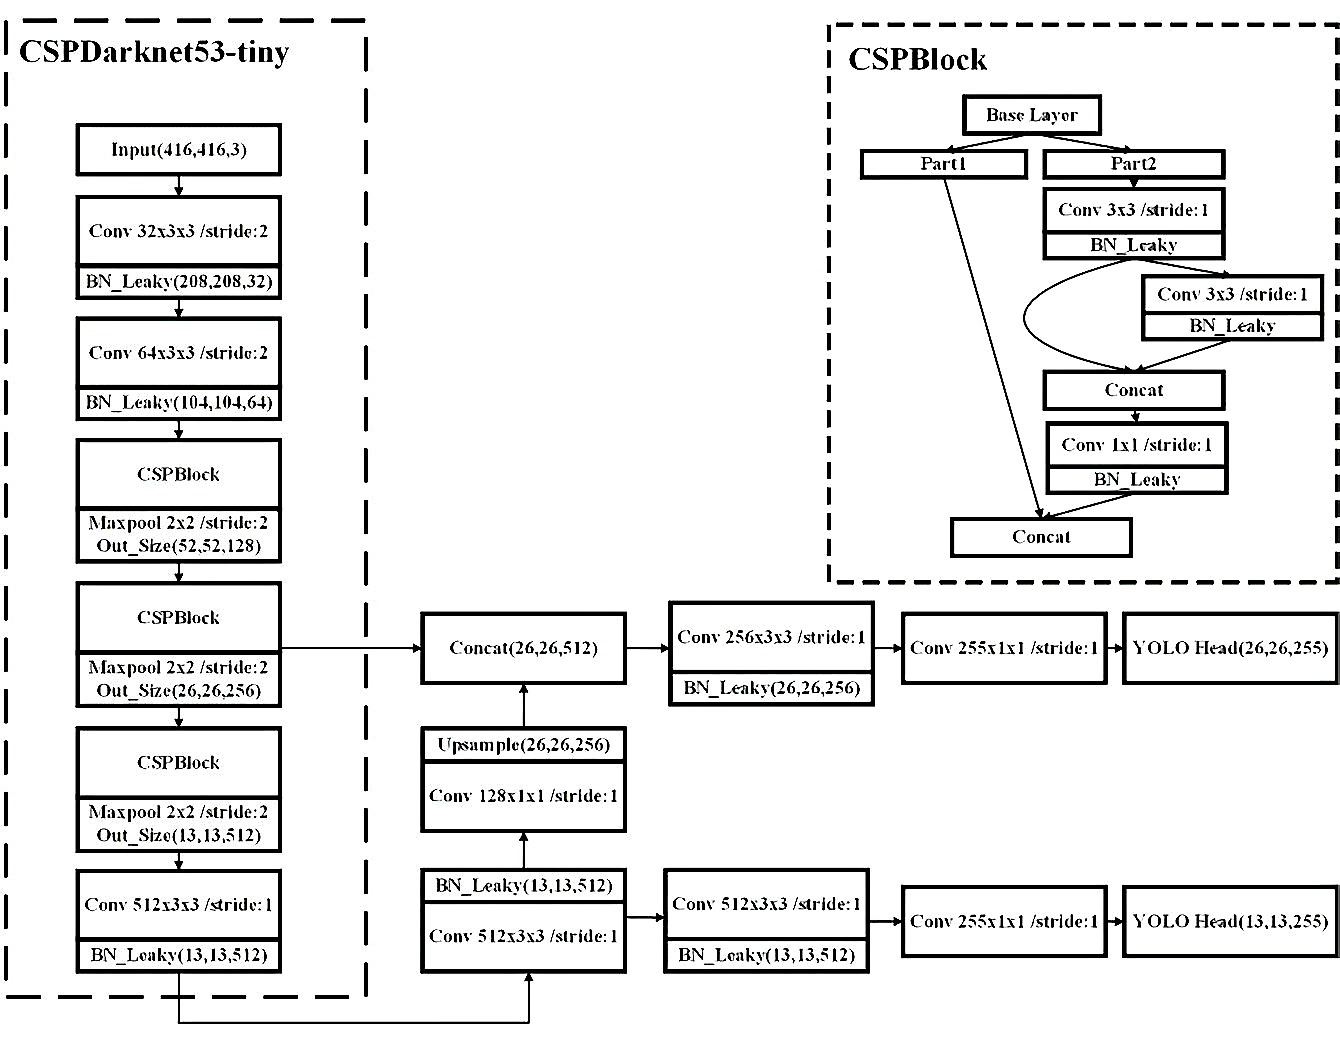
\includegraphics[width=1\textwidth]{gambar/arsitekturyolov4tiny.jpg}
		\captionof{figure}{Arsitektur YoloV4-tiny}\citep{jiang2020real}
	\end{center}
\end{sidewaysfigure}
\newpage

\section{\textit{Convolutional Neural Network (CNN)}}
\label{subsec:CNN}
Metode CNN (Convolutional Neural Network) merupakan pengembangan dari \textit{Metode
Multilayer Perceptron (MLP)} yang didesain untuk mengolah data dua dimensi. Cara kerja CNN
memiliki kesamaan pada MLP, namun dalam CNN setiap neuron dipresentasikan dalam
bentuk tiga dimensi, tidak seperti MLP yang setiap neuron hanya berukuran satu dimensi.
Terdapat beberapa arsitektur CNN yang umum digunakan. Arsitektur tersebut yaitu
LeNet, AlexNet, ZF Net, GoogLeNet, VGGNet dan ResNet. CNN terdiri dari tiga jenis layer,
yaitu convolutional layer (Conv), pooling layer (Max pooling) dan fully-connected layer (Full
Connection). Tumpukan lapisan tersebut membentuk arsitektur dari CNN.\citep{DBLP:journals/corr/OSheaN15}

\textit{Convolutional Neural Network} (Convnets/ CNN) sangat mirip
dengan jaringan saraf tiruan yang standar yang dapat divisualisasikan
sebagai kumpulan neuron atau node atau unit yang disusun sebagai
graf asiklik (graf yang tanpa adanya loop di dalamnya). CNN memiliki
ciri khas yaitu trdapat lapisan tersembunyi yang hanya terhubung ke
subset neuron di lapisan sebelumnya. Karena konektivitas tersebut,
CNN dapat mempelajari fitur secara implisit. Arsitektur CNN
menghasilkan ekstraksi fitur hirarki yaitu filter yang dilatih untuk
tujuan spesifik, misal pada lapisan pertama bisanya difokuskan pada
identifikasi tepian atau fluktuasi warna, kemudian lapisan kedua
biasanya lebih ke identifikasi bentuk, dan filter lapisan berikutnya
biasanya lebih diarahkan untuk mempelajari bagian-bagian parsialisasi
dari objek, baik yang terlihat sedikit atau sebagian maupun yang
terlihat cukup banyak serta lapisan terakhir digunakan untuk
mengidentifikasi objek.\citep{bookDL}

\subsection{\textit{Covolutional Layer}}
\begin{center}
	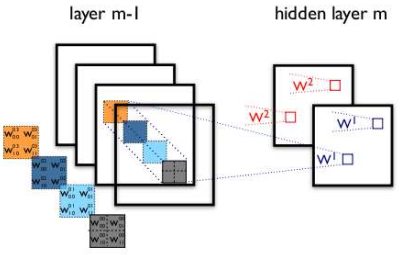
\includegraphics[width=0.75\textwidth]{gambar/konvoCNN.png}
	\captionof{figure}{Proses Konvolusi pada CNN}\citep{Wayan_Suartika_undated-rv}
	\label{fig:konvCNN}
\end{center}
Convolutional Layer merupakan proses utama dalam CNN yang
bertugas melakukan operasi konvolusi pada output dari layer sebelumnya. Konvolusi yaitu mengaplikasikan sebuah fungsi pada output fungsi lain secara berulang. Seperti pada Gambar \ref{fig:konvCNN}, konvolusi
mengaplikasikan kernel yang berwarna kuning pada citra disemua
offset. Kotak hijau secara keseluruhan adalah citra yang akan dikonvolusi. Kernel bergerak dari sudut kiri atas ke kanan bawah.
Sehingga hasil konvolusi dari citra tersebut dapat dilihat pada gambar bagian kanan.

\begin{center}
	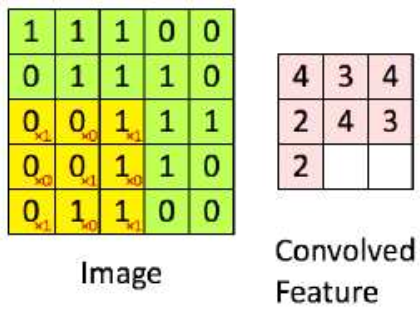
\includegraphics[width=0.75\textwidth]{gambar/ilusKonvo.png}
	\captionof{figure}{Ilustrasi Proses Konvolusi}\citep{Wayan_Suartika_undated-rv}
	\label{fig:prosKonv}
\end{center}
Tujuan dilakukannya konvolusi pada data citra adalah untuk mengekstraksi fitur dari citra input. Konvolusi akan
menghasilkan transformasi linier dari data input sesuai informasi
spasial pada data. Bobot pada layer tersebut menspesifikasikan
kernel konvolusi yang digunakan, sehingga kernel konvolusi dapat
dilatih berdasarkan input pada CNN.

\subsection{\textit{Subsampling Layer}}
Subsampling Layer adalah proses mereduksi ukuran sebuah data citra. Tujuannya untuk meningkatkan invariansi posisi dari fitur.
Dalam CNN, metode subsampling yang digunakan adalah max pooling. Pada ilustrasi pada Gambar \ref{fig:maxpool}, Max pooling membagi output
dari convolution layer menjadi beberapa grid kecil lalu mengambil
nilai maksimal dari setiap grid untuk menyusun matriks citra yang
telah direduksi. Grid yang berwarna merah, hijau, kuning dan biru merupakan kelompok grid yang akan dipilih nilai maksimumnya.
Sehingga hasil dari proses tersebut dapat dilihat pada kumpulan
grid disebelah kanannya. Proses tersebut memastikan fitur yang
didapatkan akan sama meskipun objek citra mengalami translasi
(pergeseran). Penggunaan pooling layer pada CNN hanya bertujuan untuk mereduksi ukuran citra sehingga dapat dengan mudah
digantikan dengan sebuah convolution layer dengan stride yang sama dengan pooling layer yang bersangkutan.\citep{Wayan_Suartika_undated-rv}
\begin{center}
	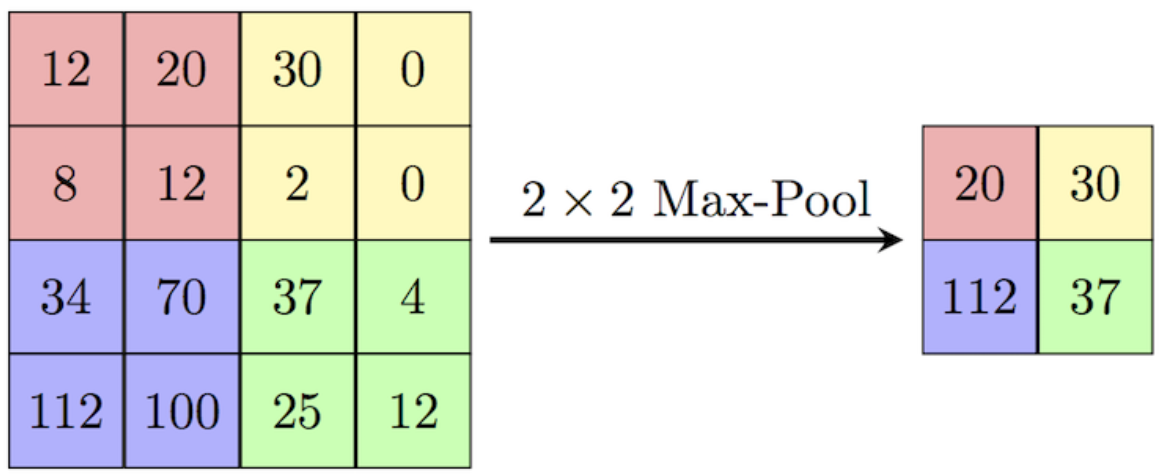
\includegraphics[width=0.75\textwidth]{gambar/ilusMaxpool.png}
	\captionof{figure}{Ilustrasi Operasi \textit{Max Pooling}}\citep{Wayan_Suartika_undated-rv}
	\label{fig:maxpool}
\end{center}

\subsection{\textit{Fully Connected Layer}}
Fully-Connected Layer bertujuan untuk melakukan transformasi pada dimensi data agar data dapat diklasifikasikan secara linier. Setiap neuron pada convolution layer perlu ditransformasi menjadi data satu dimensi terlebih dahulu sebelum dapat dimasukkan
ke dalam sebuah fully connected layer. Karena hal tersebut menyebabkan data kehilangan informasi spasialnya dan tidak reversibel,
fully connected layer hanya dapat diimplementasikan diakhir jaringan. Convolution layer dengan ukuran kernel $1 \times 1$ melakukan fungsi
yang sama dengan sebuah fully connected layer namun dengan tetap
mempertahankan karakter spasial dari data.\citep{Wayan_Suartika_undated-rv}

\section{\textit{Image Processing}}
\textit{Image Processing} atau Pengolahan Citra merupakan teknik
dalam pemrosesan gambar dengan input berupa citra dua dimensi yang bertujuan untuk menyempurnakan citra atau mendapatkan
informasi yang berguna untuk diolah menjadi beberapa keputusan. Dalam operasi pemrosesan citra, operasi yang sering dilakukan
dalam gambar grayscale. Gambar grayscale didapatkan dari pemrosesan gambar berwarna yang didekomposisi menjadi komponen
merah (R), hijau (G) dan biru (B) yang diproses secara independen
sebagai gambar grayscale. Image Processing terbagi menjadi dalam 3 tingkatan\citep{bookDigiPro}:
\begin{enumerate}
	\item \textit{Low-Level Image Processing}\\
	Low-Level Image Processing merupakan operasi sederhana dalam pengolahan gambar dimana input dan output berupa gambar. Contoh: contrast enchancement dan noise reduction.\citep{bookDigiPro}
	\item \textit{Mid-Level Image Processing}\\
	Mid-Level Image Processing merupakan operasi pengolahan
	gambar yang melibatkan ekstrasi atribut dari gambar input.
	Contoh: edges, contours dan regions.\citep{bookDigiPro}
	\item \textit{High-Level Image Processing}\\
	High-Level Image Processing merupakan merupakan kategori
	yang melibatkan pemrosesan gambar kompleks yang terkait
	dengan analisis dan interpretasi konten dalam sebuah keadaan
	untuk pengambilan keputusan.\citep{bookDigiPro}
\end{enumerate}

\subsection{\textit{Digital Image}}
Digital Image merupakan fungsi dua dimensi f(x,y) yang merupakan proyeksi dari bentuk tiga dimensi kedalam bentuk dua dimensi dimana x dan y merupakan lokasi elemen gambar atau piksel yang berisikan nilai. Ketika nilai x,y dan intensitasnya berupa
diskrit, maka gambar tersebut dapat dikategorikan sebagai digital
image. Secara matematis, digital image adalah representasi matriks
dari gambar dua dimensi menggunakan piksel. Setiap piksel diwakili oleh nilai numerik. Untuk gambar grayscale, hanya memiliki satu
nilai dengan kisaran antara 0-255.Pada Gambar \ref{fig:digipro}, untuk gambar yang berwarna, memiliki tiga nilai yang mewakili merah (R),
hijau (G) dan biru (B) yang masing-masing memiliki kisaran nilai
yang sama antara 0-255. Jika suatu gambar hanya memiliki dua
intensitas, gambar tersebut dikenal sebagai binary image.\citep{bookDigiPro}

\begin{center}
	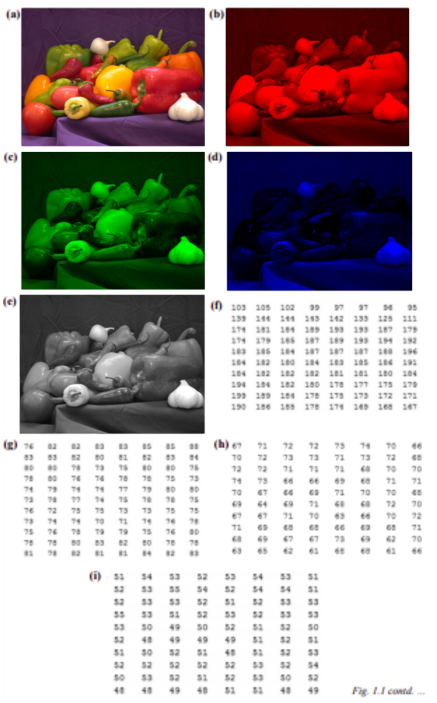
\includegraphics[width=0.69\textwidth]{gambar/digipro.png}
	\captionof{figure}{(a) Gambar berwarna, (b) Komponen merah dalam gambar berwarna, (c) Komponen hijau dalam gambar bewarna, (d) Komponen biru dalam gambar bewarna, (e) Gambar bewarna dikonversi dalam
		8-bit grayscale, (f) Matriks dari gambar (b), (g) Matriks dari gambar (c),
		(h) Matriks dari gambar (d), (i) Matriks dari gambar (e)}\citep{bookDigiPro}
	\label{fig:digipro}
\end{center}



